% TMLR submission. Anonymous: \usepackage{tmlr} with no options.
% For camera-ready use \usepackage[accepted]{tmlr}; for a preprint, [preprint].
% Style files (tmlr.sty, tmlr.bst, fancyhdr.sty) are vendored in this directory
% from https://github.com/JmlrOrg/tmlr-style-file.
\documentclass[10pt]{article}
\usepackage{tmlr}

\usepackage{booktabs}
\usepackage{graphicx}
\usepackage{amsmath}
\usepackage{amssymb}
\usepackage{url}
\graphicspath{{../figs/}}

\title{Pyramidal wrappers break non-abstaining dense matchers:\\
a diagnostic study of foundation-model registration\\
in correlative microscopy}

\author{\name Anonymous Author(s) \email anon@example.com \\
      \addr Anonymous Institution}

\def\month{08}
\def\year{2026}
\def\openreview{\url{https://openreview.net/forum?id=XXXXXXXXXX}}

\begin{document}

\maketitle

\begin{abstract}
Correlative microscopy pairs images of one specimen across modalities (SEM, EBSD, TEM, optical) that share little appearance and can differ in field of view (FOV) by orders of magnitude. A natural training-free remedy is to wrap a pretrained dense matcher in an image pyramid: tile the wide-FOV image, match each tile, pool the correspondences, and fit one global transform. We show that this fails for a structural reason. Dense matchers do not abstain --- every tile returns on the order of $10^4$ confident correspondences whether or not it overlaps the target --- so pooling floods robust estimation with mostly-spurious matches, collapsing the median inlier fraction from 0.114 to 0.005 and RoMa's median error from 80 to 2708\,px, with 106 of 187 pairs becoming hard failures. A verified coarse-to-fine wrapper, which admits a candidate transform only when a mutual-information verifier beats the incumbent, removes the collapse but buys nothing in aggregate on the benchmark (SR@10 $0.091\rightarrow0.091$): it converts one low-FOV failure into a success and loses one high-FOV success, which is the trade its scale mechanism predicts. To test that mechanism in isolation we build a controlled FOV ladder that crops real pairs while holding appearance, modality and pixel size fixed; there the wrapper triples success at 10\,\% FOV ($0.075\rightarrow0.225$, $p=0.0028$; $0.045\rightarrow0.227$ on pairs held out of fine-tuning, $p=0.023$). The benchmark simply never presents scale as an isolated failure mode: a directly measured appearance axis (normalised mutual information on the ground-truth-aligned overlap) confirms that low-FOV pairs are also the most appearance-divergent ($r=+0.215$, $p=0.003$), and with at most three of 61 sub-0.5-area-ratio pairs ever registered by any zero-shot or wrapped configuration there is too little leverage to rank scale against appearance. Decoder-only domain fine-tuning cuts in-distribution error ${\sim}5\times$ but, across eight runs, regresses held-out SR@20 ($0.393\rightarrow0.26$) on the single modality combination absent from training, and an L2-SP weight anchor does not fix it. Finally we report a methodological hazard that we did not anticipate: scoring the identical experiments after an optional thin-plate-spline refinement stage, whose coverage ranges from 0.000 to 1.000 across configurations, turns both of our null aggregate results into significant ones ($p=0.034$ and $p=0.035$). We therefore headline the unrefined parametric error and report both throughout.
\end{abstract}

\section{Introduction}

Correlative microscopy spatially associates measurements of a single specimen acquired by different instruments: scanning electron microscopy (SEM), electron backscatter diffraction (EBSD), transmission electron microscopy (TEM), light microscopy (LOM), and derived modalities such as image-quality and inverse-pole-figure maps. Linking a dislocation configuration in TEM to a grain orientation in EBSD requires bringing two images into a common coordinate frame to sub-grain precision, and registration is the bottleneck \citep{durmaz2026foundation}. The regime couples two compounding difficulties. The modalities share little mutual information, because a secondary-electron contrast image and a crystallographic orientation map are produced by entirely different physics. And the field of view (FOV) can differ by more than an order of magnitude, with the narrow-FOV image covering as little as 2\,\% of the wide-FOV frame. Classical intensity- and feature-based methods assume shared appearance and comparable scale, and fail outright \citep{durmaz2026amalgamatch}.

Learned dense matchers have transformed correspondence estimation for natural images. Detector-free transformers such as LoFTR \citep{sun2021loftr} and its efficient successor \citep{wang2024efficientloftr} produce semi-dense matches in texture-poor scenes; RoMa \citep{edstedt2024roma} couples frozen DINOv2 features \citep{oquab2024dinov2} with a fine-feature branch and a match-classification decoder to yield pixel-dense warps with calibrated certainty; and MatchAnything \citep{he2025matchanything} retrains such backbones on large-scale synthetic cross-modal signal. One property of this family is central to what follows. Sparse learned matchers built on keypoint detection and attention-based assignment \citep{sarlin2020superglue,lindenberger2023lightglue} can decline to match. Detector-free dense matchers instead emit a confident correspondence at essentially every pixel and \emph{never abstain}.

The obvious way to spend that density on a FOV gap is a pyramid: crop the wide-FOV source into target-resolution tiles, match each tile, pool the correspondences, and fit one global transform by robust estimation. It requires no training and treats the matcher as a black box. This paper reports what happens when that idea is executed carefully on all 187 pairs of the AmalgaMatch benchmark, and the result is diagnostic rather than methodological. Our contributions are:

\begin{enumerate}
\item \textbf{A mechanism.} The naive pyramid does not merely fail to help; it destroys the backbone it wraps, and it does so because dense matchers do not abstain (Section~\ref{sec:v1}). Non-overlapping tiles contribute confident garbage, the inlier fraction collapses by a factor of 22, and the robust estimator has no consensus to find. This predicts failure for \emph{any} pool-then-fit pyramid over a non-abstaining matcher, independent of tile size or overlap.
\item \textbf{A wrapper that survives, and an honest account of what it buys.} A verified coarse-to-fine design removes the collapse (Section~\ref{sec:v2}), but on the native benchmark its aggregate effect is exactly zero. What it does is shift \emph{which} pairs succeed, in the direction its mechanism predicts.
\item \textbf{A controlled decoupling.} A FOV ladder that crops real pairs with appearance held fixed shows the scale mechanism is sound where scale is the isolated variable (Section~\ref{sec:ladder}), and a directly measured appearance axis shows why the native benchmark cannot show this: scale and appearance are confounded on it, and it carries too little leverage below area ratio 0.5 to separate them (Section~\ref{sec:appearance}).
\item \textbf{A methodological hazard.} An optional refinement stage with non-uniform coverage across configurations converts both of our null results into significant ones (Section~\ref{sec:metric}). We report the consequences for our own claims in full, and argue the failure mode is general.
\end{enumerate}

The original project hypotheses were (H1) that pyramidal patching yields ${\ge}35\,\%$ relative gain at FOV\,${\le}\,5\,\%$ over the best zero-shot baseline; (H2) that RoMa's dense flow tolerates partial overlap better than the ELoFTR family at low FOV; and (H3) that an affine model suffices for AmalgaMatch, with full homography offering no significant benefit. We state verdicts on all three in Section~\ref{sec:verdicts}.

\section{Related work}

\paragraph{Dense and detector-free matching.} LoFTR \citep{sun2021loftr} replaced keypoint detection with coarse-to-fine attention over feature grids, and Efficient LoFTR \citep{wang2024efficientloftr} reduced its cost. RoMa \citep{edstedt2024roma} is dense rather than semi-dense: it regresses a warp at every pixel together with a certainty map, using frozen DINOv2 features \citep{oquab2024dinov2} for robustness and a separate fine-feature branch for precision. The certainty map is the natural place for an abstention signal, and Section~\ref{sec:v2} reports an ablation that gates on it; the gate makes matters worse, because on hard pairs everything is low-certainty.

\paragraph{Cross-modal generalisation.} MatchAnything \citep{he2025matchanything} trains matcher architectures on large-scale synthetic cross-modality signal and reports strong zero-shot transfer across unseen modality pairs with a single weight set. We evaluate both its ELoFTR and its RoMa variants. Sparse learned matchers \citep{sarlin2020superglue,lindenberger2023lightglue} sit outside our scope precisely because they can abstain, which is the property whose absence drives our central negative result.

\paragraph{Registration in correlative microscopy.} \citet{durmaz2026amalgamatch} introduced AmalgaMatch and reported that classical registration fails on it; \citet{durmaz2026foundation} evaluated foundation matchers on the same data and found MatchAnything-RoMa the strongest configuration across most subsets. Our aggregate ordering agrees with theirs. What we add is a mechanism for the wrapper class, a controlled protocol that separates scale from appearance, and a measurement of how the choice of error metric changes the conclusions.

\paragraph{Fine-tuning without forgetting.} Section~\ref{sec:finetune} adapts a matcher to the materials domain and observes catastrophic forgetting \citep{kirkpatrick2017ewc} of an untrained modality combination. We test L2-SP \citep{li2018l2sp}, a one-line penalty anchoring weights to their pretrained values, as the cheapest available remedy. Parameter-efficient alternatives such as LoRA \citep{hu2022lora} would constrain the update differently and are not evaluated here.

\section{Setting}
\label{sec:setting}

\paragraph{Benchmark.} AmalgaMatch \citep{durmaz2026amalgamatch} contains 187 image pairs spanning six correlative-microscopy task groups (orientation mapping, serial sectioning, multiscale, slip partitioning, fracture surfaces, dislocation characterisation) across 19 material subsets, each pair carrying ground-truth (GT) point correspondences.

\paragraph{Pipeline.} Per pair we match, fit a transform with MAGSAC++ \citep{barath2020magsac} at a 5.5\,px reprojection threshold, selecting affine against homography by a BIC-style penalty on inlier residuals. Accuracy is the mean Euclidean distance (ED) between GT target points mapped into source coordinates and their GT source positions. Aggregates are median ED and success rates SR@$\{5,10,20\}$\,px.

\paragraph{Error metric.} The pipeline optionally refines the fitted transform on its inliers with a thin-plate spline (TPS) \citep{bookstein1989tps}. \textbf{We report the unrefined parametric error as the primary metric} and the refined error alongside. This is a deliberate reversal of our original protocol, and Section~\ref{sec:metric} gives the evidence: TPS coverage ranges from 0.000 to 1.000 across configurations, so a TPS-scored table compares some configurations under refined error and others under raw error. The unrefined metric scores every configuration identically. Note the direction of the change: it removes statistical significance from two results rather than creating it.

\paragraph{FOV strata.} We bin pairs by GT-implied target/source area ratio with edges ${<}0.05$ ($n=4$), 0.05--0.25 ($n=33$), 0.25--0.5 ($n=24$) and ${\ge}0.5$ ($n=126$), calling the first two the \emph{extreme}- and \emph{low}-FOV strata. Earlier drafts used ``severe'' for both and we avoid the word here. Only four pairs sit below ratio 0.05 under any definition, so no claim resting on that stratum alone can carry weight.

\paragraph{A protocol floor.} The GT itself fits a global affine only to ${\sim}10.3$\,px median residual. Threshold metrics are therefore floored well above the sub-pixel precision the original plan assumed, and any sub-5\,px claim on AmalgaMatch measures the GT more than the method. We report SR@5 for completeness and rest no conclusion on it.

\paragraph{Statistics.} Method-vs-method comparisons use a paired bootstrap over per-pair errors ($B=10{,}000$) with 95\,\% percentile confidence intervals on the difference of the relevant aggregate. Reported $p$-values are two-sided, computed as twice the smaller tail mass of the bootstrap difference distribution and capped at 1. Success-rate proportions carry Wilson score intervals, which behave correctly near zero; several strata here sit at or near zero.

\begin{table}[t]
\centering
\small
\begin{tabular}{lrrrrr}
\toprule
Configuration & med ED (px) & SR@5 & SR@10 & SR@20 & fits \\
\midrule
SIFT (Control A)                & 903.1  & 0.011 & 0.016 & 0.021 & 169/187 \\
SIFT + MI (Control B)           & 823.6  & 0.011 & 0.016 & 0.021 & 169/187 \\
LoFTR                           & 270.1  & 0.037 & 0.064 & 0.091 & 183/187 \\
MatchAnything-ELoFTR            & 510.1  & 0.011 & 0.011 & 0.032 & 177/187 \\
RoMa (zero-shot)                & 80.2   & 0.059 & 0.091 & 0.225 & 187/187 \\
RoMa + pyramid v1               & 2707.6 & 0.000 & 0.005 & 0.021 & \phantom{0}81/187 \\
RoMa + pyramid v2               & \textbf{69.9} & 0.059 & 0.091 & 0.219 & 187/187 \\
MatchAnything-RoMa              & 81.0   & 0.059 & 0.107 & 0.241 & 187/187 \\
MatchAnything-RoMa + pyramid v2 & 77.6   & 0.053 & \textbf{0.118} & 0.230 & 187/187 \\
\bottomrule
\end{tabular}
\caption{\textbf{Registration accuracy on all 187 AmalgaMatch pairs, unrefined parametric error.} ``fits'' counts pairs on which the estimator returned a transform at all; the remainder are scored as failures at every threshold. Classical methods reproduce the benchmark's near-total failure. The naive pyramid (v1) destroys RoMa. The verified wrapper (v2) restores it but adds nothing in aggregate. No difference among the four dense rows is statistically significant on this metric (Section~\ref{sec:metric}, Table~\ref{tab:contrasts}); under the TPS-refined metric two of them are. The fine-tuned backbone is excluded from this table because it was trained on 131 of these 187 pairs; it appears only in Section~\ref{sec:finetune}.}
\label{tab:headline}
\end{table}

\paragraph{Baselines.} Table~\ref{tab:headline} reports the headline comparison, and Figure~\ref{fig:srbars} the same data with Wilson intervals. Classical baselines reproduce the benchmark's own finding: SIFT \citep{lowe2004sift} succeeds on 3 of 187 pairs, and mutual-information intensity refinement \citep{maes1997mutualinfo} moves median ED by ${\sim}80$\,px without flipping a single pair to success. Among zero-shot foundation matchers RoMa is the strongest single backbone, and MatchAnything-RoMa is nominally stronger still.

\section{Pooling breaks non-abstaining matchers}
\label{sec:v1}

The direct implementation of the scale hypothesis (pyramid v1) tiles the source into a sliding-window pyramid at 50\,\% overlap whose levels match the target's nominal physical resolution, matches every tile against the target, back-projects and pools all correspondences, then fits one global transform. It does not help. It destroys the backbone.

RoMa's median error rises from 80.2 to 2707.6\,px and 106 of 187 pairs become hard failures, meaning the estimator cannot return a transform at all (Table~\ref{tab:headline}). The mechanism is structural. RoMa returns exactly $10^4$ correspondences per invocation on all 187 pairs --- a fixed sampling cap, hit every time --- and it returns them whether or not the tile overlaps the target at all, because it has no mechanism for declining. Pooling over a pyramid therefore contributes one honest tile's worth of signal and $k-1$ tiles' worth of confident noise. The pooled counts make the scale of the flood concrete: pyramid v1 reaches 9{,}420{,}000 correspondences on a single pair, or 942 tiles' worth, of which at most one tile's worth can be correct. Measured over all 187 pairs, the median inlier fraction falls from 0.114 for the direct match to 0.005 for the pyramid, a factor of 22. MAGSAC++ is a marginalising estimator in the RANSAC lineage \citep{fischler1981ransac,barath2020magsac} and is robust to a minority of outliers; at a 0.5\,\% inlier fraction there is no consensus set left to find.

We stress that this is a property of the class, not a tuning artefact. The argument makes no reference to tile size, overlap fraction, pyramid depth, or the particular backbone: any pool-then-fit scheme over a matcher that cannot abstain will contribute outliers in proportion to the number of non-overlapping tiles, and the inlier fraction will fall roughly as the reciprocal of the tile count. The remedy is not a better pyramid but a mechanism that decides \emph{which} tile to believe before pooling anything --- which is what the next section builds.

\begin{figure}[t]
\centering
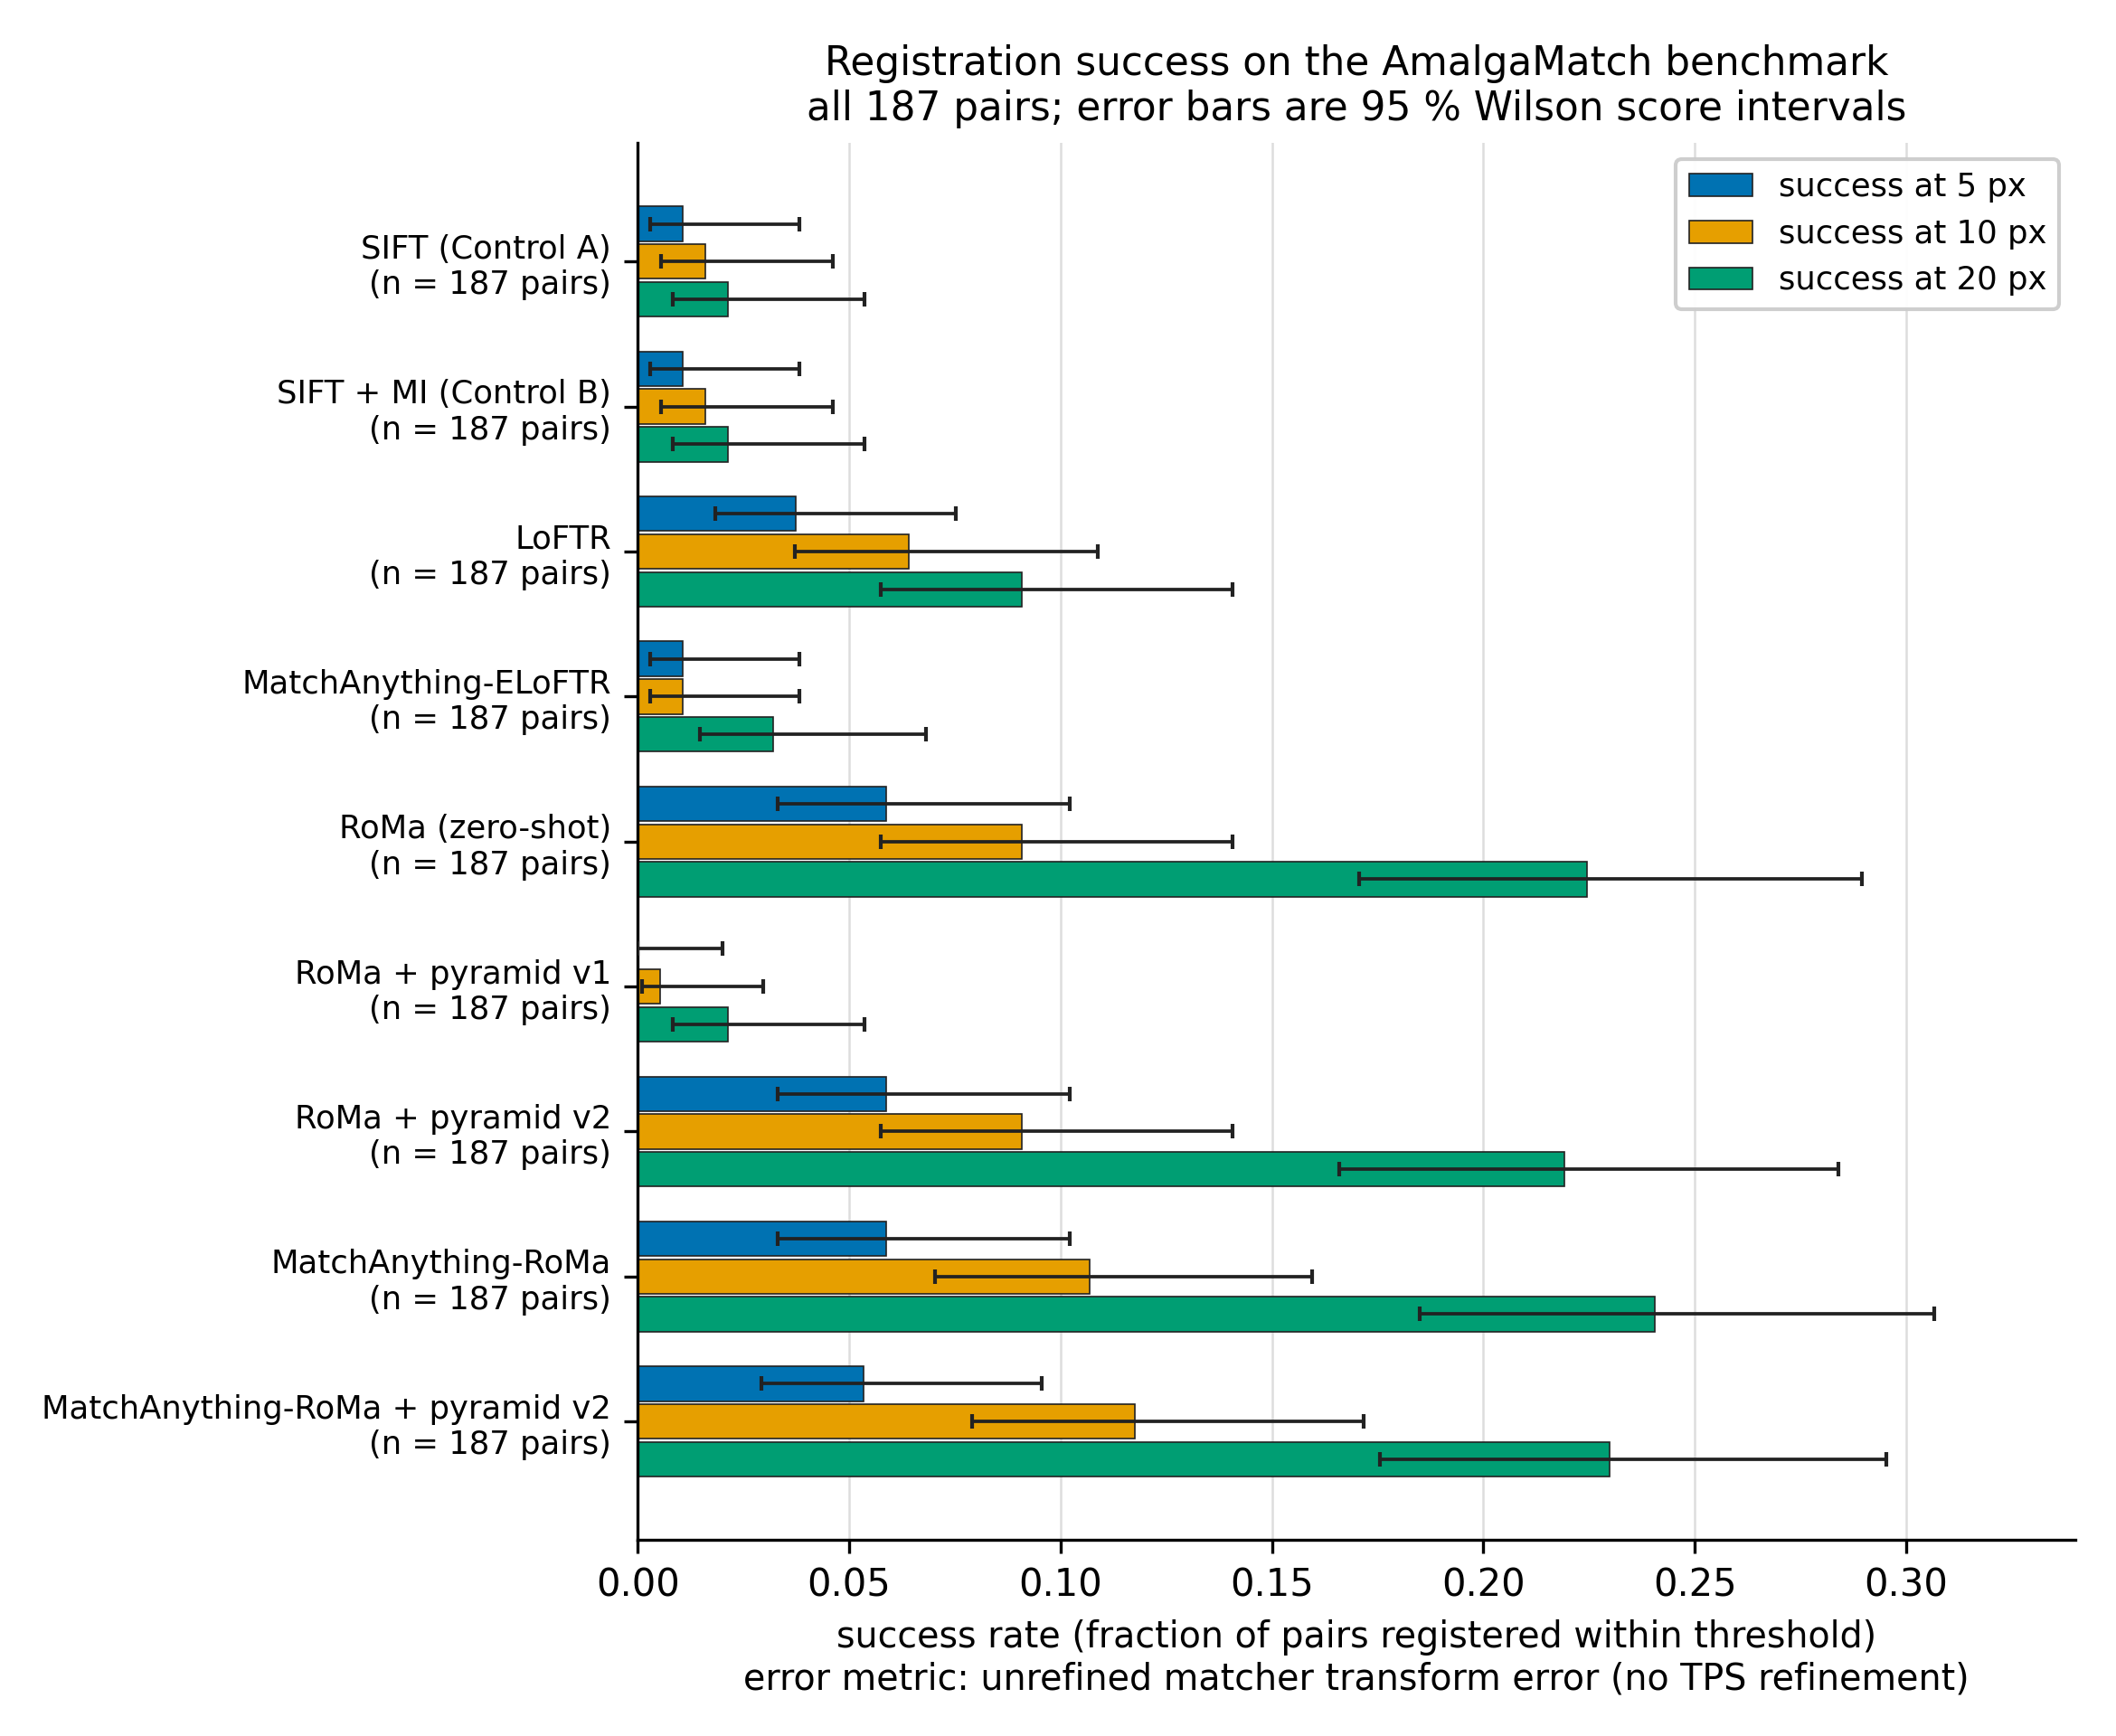
\includegraphics[width=\linewidth]{sr_bars_raw.png}
\caption{\textbf{Success rates across all nine configurations, unrefined parametric error, all 187 pairs.} Error bars are 95\,\% Wilson score intervals. Pyramid v1 collapses RoMa; pyramid v2 restores it to parity. The intervals overlap throughout the dense-matcher rows, which is the honest summary of the native-pair comparison: nothing here is separated. Figure~\ref{fig:metric} shows the same panel under the refined metric, where two contrasts become significant.}
\label{fig:srbars}
\end{figure}

\section{A verified coarse-to-fine wrapper, and what it does not buy}
\label{sec:v2}

We redesigned the wrapper so that it never pools blindly (pyramid v2; Figure~\ref{fig:schematic}a). It matches the full pair directly first, giving an incumbent transform. It invokes candidate stages --- tile search over a scaled source grid, then zoom refinement on the best-scoring region --- only when direct support is weak, and it accepts a candidate only if a mutual-information-on-overlap verifier scores it above the incumbent. The design is therefore monotone with respect to its own verifier: tile noise cannot displace a direct fit the verifier prefers.

This removes the collapse completely. RoMa + pyramid v2 restores all 187 fits and improves median error from 80.2 to 69.9\,px ($-10.3$\,px, 95\,\% CI $[-48.2,+23.2]$, $p=0.37$). But on the native benchmark that is the whole story: the aggregate success rate is unchanged, SR@10 $0.091\rightarrow0.091$ (95\,\% CI $[-0.016,+0.016]$, $p=1.00$), and SR@20 is nominally lower ($0.225\rightarrow0.219$, $p=0.83$). \textbf{The wrapper buys nothing in aggregate.}

What it does is change which pairs succeed, and the direction is exactly what its mechanism predicts. Counting successes by FOV stratum (Table~\ref{tab:strata}), the wrapper converts one low-FOV failure into a success (1/33 $\rightarrow$ 2/33 in the 0.05--0.25 stratum) and loses one high-FOV success (15/126 $\rightarrow$ 14/126). Seventeen pairs succeed either way; the composition shifts and the total does not. A wrapper whose only mechanism is scale search should help where FOV is the binding constraint and cost a little where it is not, on a benchmark where 126 of 187 pairs are already at comparable scale. That is what we measure. The effect is two pairs wide and we draw no inference from its statistical significance, of which it has none; we report it because the sign structure is a prediction the mechanism makes and could have failed.

\begin{table}[t]
\centering
\small
\begin{tabular}{lcccc}
\toprule
& \multicolumn{4}{c}{SR@10 by FOV area ratio (successes / pairs)} \\
\cmidrule(lr){2-5}
Configuration & ${<}0.05$ ($n{=}4$) & 0.05--0.25 ($n{=}33$) & 0.25--0.5 ($n{=}24$) & ${\ge}0.5$ ($n{=}126$) \\
\midrule
SIFT (Control A)                & 0/4 & 0/33 & 1/24 & \phantom{0}2/126 \\
SIFT + MI (Control B)           & 0/4 & 0/33 & 1/24 & \phantom{0}2/126 \\
LoFTR                           & 0/4 & 0/33 & 1/24 & 11/126 \\
MatchAnything-ELoFTR            & 0/4 & 0/33 & 0/24 & \phantom{0}2/126 \\
RoMa (zero-shot)                & 0/4 & 1/33 & 1/24 & 15/126 \\
RoMa + pyramid v1               & 0/4 & 0/33 & 0/24 & \phantom{0}1/126 \\
RoMa + pyramid v2               & 0/4 & \textbf{2/33} & 1/24 & 14/126 \\
MatchAnything-RoMa              & 0/4 & 0/33 & 1/24 & 19/126 \\
MatchAnything-RoMa + pyramid v2 & 0/4 & 1/33 & 1/24 & \textbf{20/126} \\
\bottomrule
\end{tabular}
\caption{\textbf{Success at 10\,px by native FOV stratum, unrefined error.} Every configuration is at the floor in the extreme-FOV stratum. The wrapper's low-FOV gain and high-FOV loss on RoMa are visible as $1\rightarrow2$ and $15\rightarrow14$. Across the 61 pairs below area ratio 0.5, no configuration registers more than three. Figure~\ref{fig:fovcurves} plots these with intervals.}
\label{tab:strata}
\end{table}

\paragraph{Ablations.} Two ablations show the design is at its useful limit. Iterated zoom, which chains refinements, is not significantly better than a single zoom and is borderline worse, because each stage compounds verifier error. Certainty gating at 0.5, which discards low-certainty matches before fitting, does not help either: on the unrefined metric it is exactly null (SR@20 $0.219\rightarrow0.219$, 95\,\% CI $[-0.021,+0.021]$, $p=1.00$), and on the refined metric it is significantly \emph{worse} than plain v2 ($-0.037$, 95\,\% CI $[-0.070,-0.011]$, $p=0.002$). The gate never improves on either metric, and it starves the estimator on exactly the hard pairs where every match is low-certainty. This is worth stating plainly given the framing of Section~\ref{sec:v1}: RoMa's certainty map is the obvious candidate for the abstention signal whose absence causes the collapse, and thresholding it does not recover the missing behaviour.

\paragraph{The verifier ceiling.} On the stronger MatchAnything-RoMa backbone the wrapper again produces no significant aggregate change (SR@10 $0.107\rightarrow0.118$, $\Delta=+0.011$, 95\,\% CI $[+0.000,+0.027]$, $p=0.26$; SR@20 $-0.011$, $p=0.46$). The per-pair changes show what it is doing: exactly two pairs cross the 10\,px line and none are lost, one a marginal $11.8\rightarrow8.3$\,px and one a genuine recovery from a coarse failure at $325.8\rightarrow8.1$\,px. That split is the wrapper's competence and its ceiling in one line. A mutual-information verifier can tell a wrong region from a right one, so it rescues coarse failures; it cannot discriminate between two transforms that already agree to within ${\sim}10$\,px, so on a backbone that is mostly either right or hopeless it finds few pairs to act on. That bounds what any verifier-gated wrapper of this kind can deliver once the backbone is good.

\begin{figure}[t]
\centering
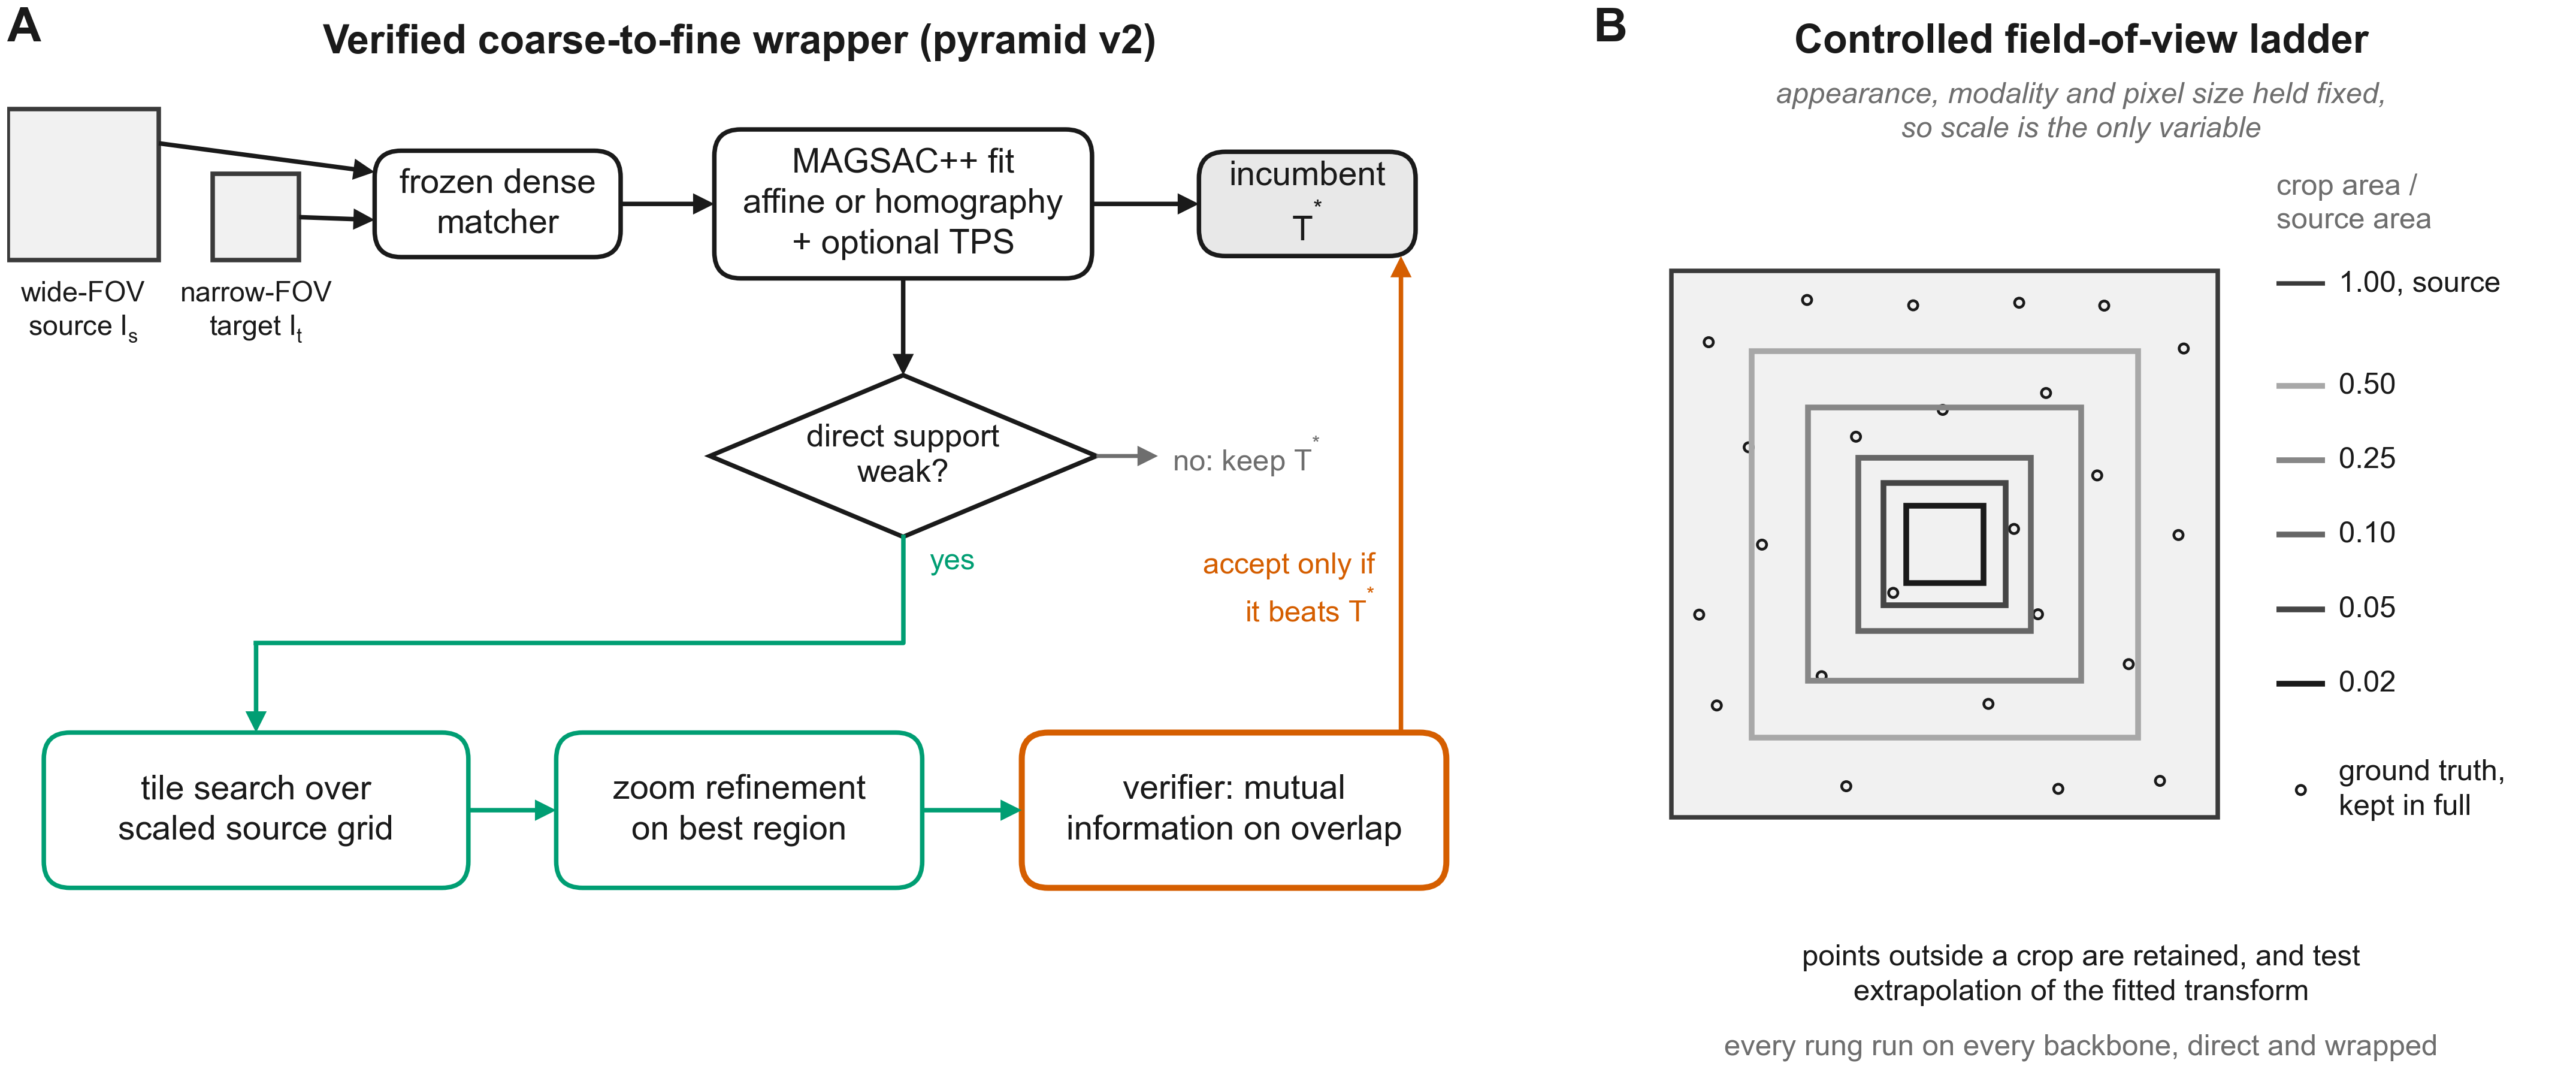
\includegraphics[width=\linewidth]{method_schematic.png}
\caption{\textbf{Method overview.} (\textbf{a}) The verified coarse-to-fine wrapper (pyramid v2): a direct match yields an incumbent transform; candidate tile-search and zoom stages are invoked only on weak support and accepted only when a mutual-information-on-overlap verifier beats the incumbent. (\textbf{b}) The FOV-ladder protocol crops real base-matchable pairs to shrinking field-of-view ratios with appearance, modality and pixel size held fixed, isolating scale as the only variable.}
\label{fig:schematic}
\end{figure}

\section{Isolating scale: a controlled FOV ladder}
\label{sec:ladder}

Section~\ref{sec:v2} leaves an ambiguity that the native benchmark cannot resolve. Either the wrapper's scale mechanism does not work, or it works and the benchmark does not present scale as an isolated failure mode. Distinguishing these requires a dataset where FOV varies and everything else does not, and AmalgaMatch is not that dataset: its low-FOV pairs are also its most appearance-divergent, and only four pairs sit below area ratio 0.05.

We therefore construct one (Figure~\ref{fig:schematic}b). For each backbone we take its \emph{base-matchable} pairs --- those the backbone registers to better than 20\,px at full FOV --- and crop the target to absolute area ratios $\{0.5,0.25,0.1,0.05,0.02\}$. Appearance, modality gap and pixel size are fixed by construction; only FOV changes. All GT is retained for evaluation, so out-of-crop correspondences test the fitted global transform's extrapolation rather than its interpolation. Base-matchability is computed per backbone, giving 38 pairs for RoMa, 41 for MatchAnything-RoMa and 53 for the fine-tuned backbone, of which 34--51 are usable at a given rung.

With scale thus isolated, the wrapper works (Figure~\ref{fig:fovladder}). On MatchAnything-RoMa at the 0.1 rung, success at 10\,px rises from 0.075 to 0.225 --- a tripling --- with $\Delta=+0.150$, 95\,\% CI $[+0.050,+0.275]$, $p=0.0028$ ($n=40$). This is the largest and most robust effect in the study. It survives the obvious objection that the ladder testbed overlaps the fine-tuning training split: restricted to pairs held out of fine-tuning the same contrast is $0.045\rightarrow0.227$, $\Delta=+0.182$, 95\,\% CI $[+0.045,+0.364]$, $p=0.023$ ($n=22$). The effect is specific to the rung where scale becomes binding: at 0.5 and 0.25 direct matching still works and the wrapper adds nothing ($p=0.73$ and $p=0.73$), and by 0.02 both have collapsed to the floor.

Two conclusions follow. First, the wrapper's mechanism is sound: given a FOV gap and nothing else, verified coarse-to-fine search recovers registrations that direct matching loses. Second, and more consequentially for anyone reading Table~\ref{tab:headline} as a verdict on the idea, \textbf{the native benchmark's null result is not evidence that the mechanism fails}. It is evidence that the mechanism addresses a failure mode the benchmark rarely presents in isolation.

\begin{figure}[t]
\centering
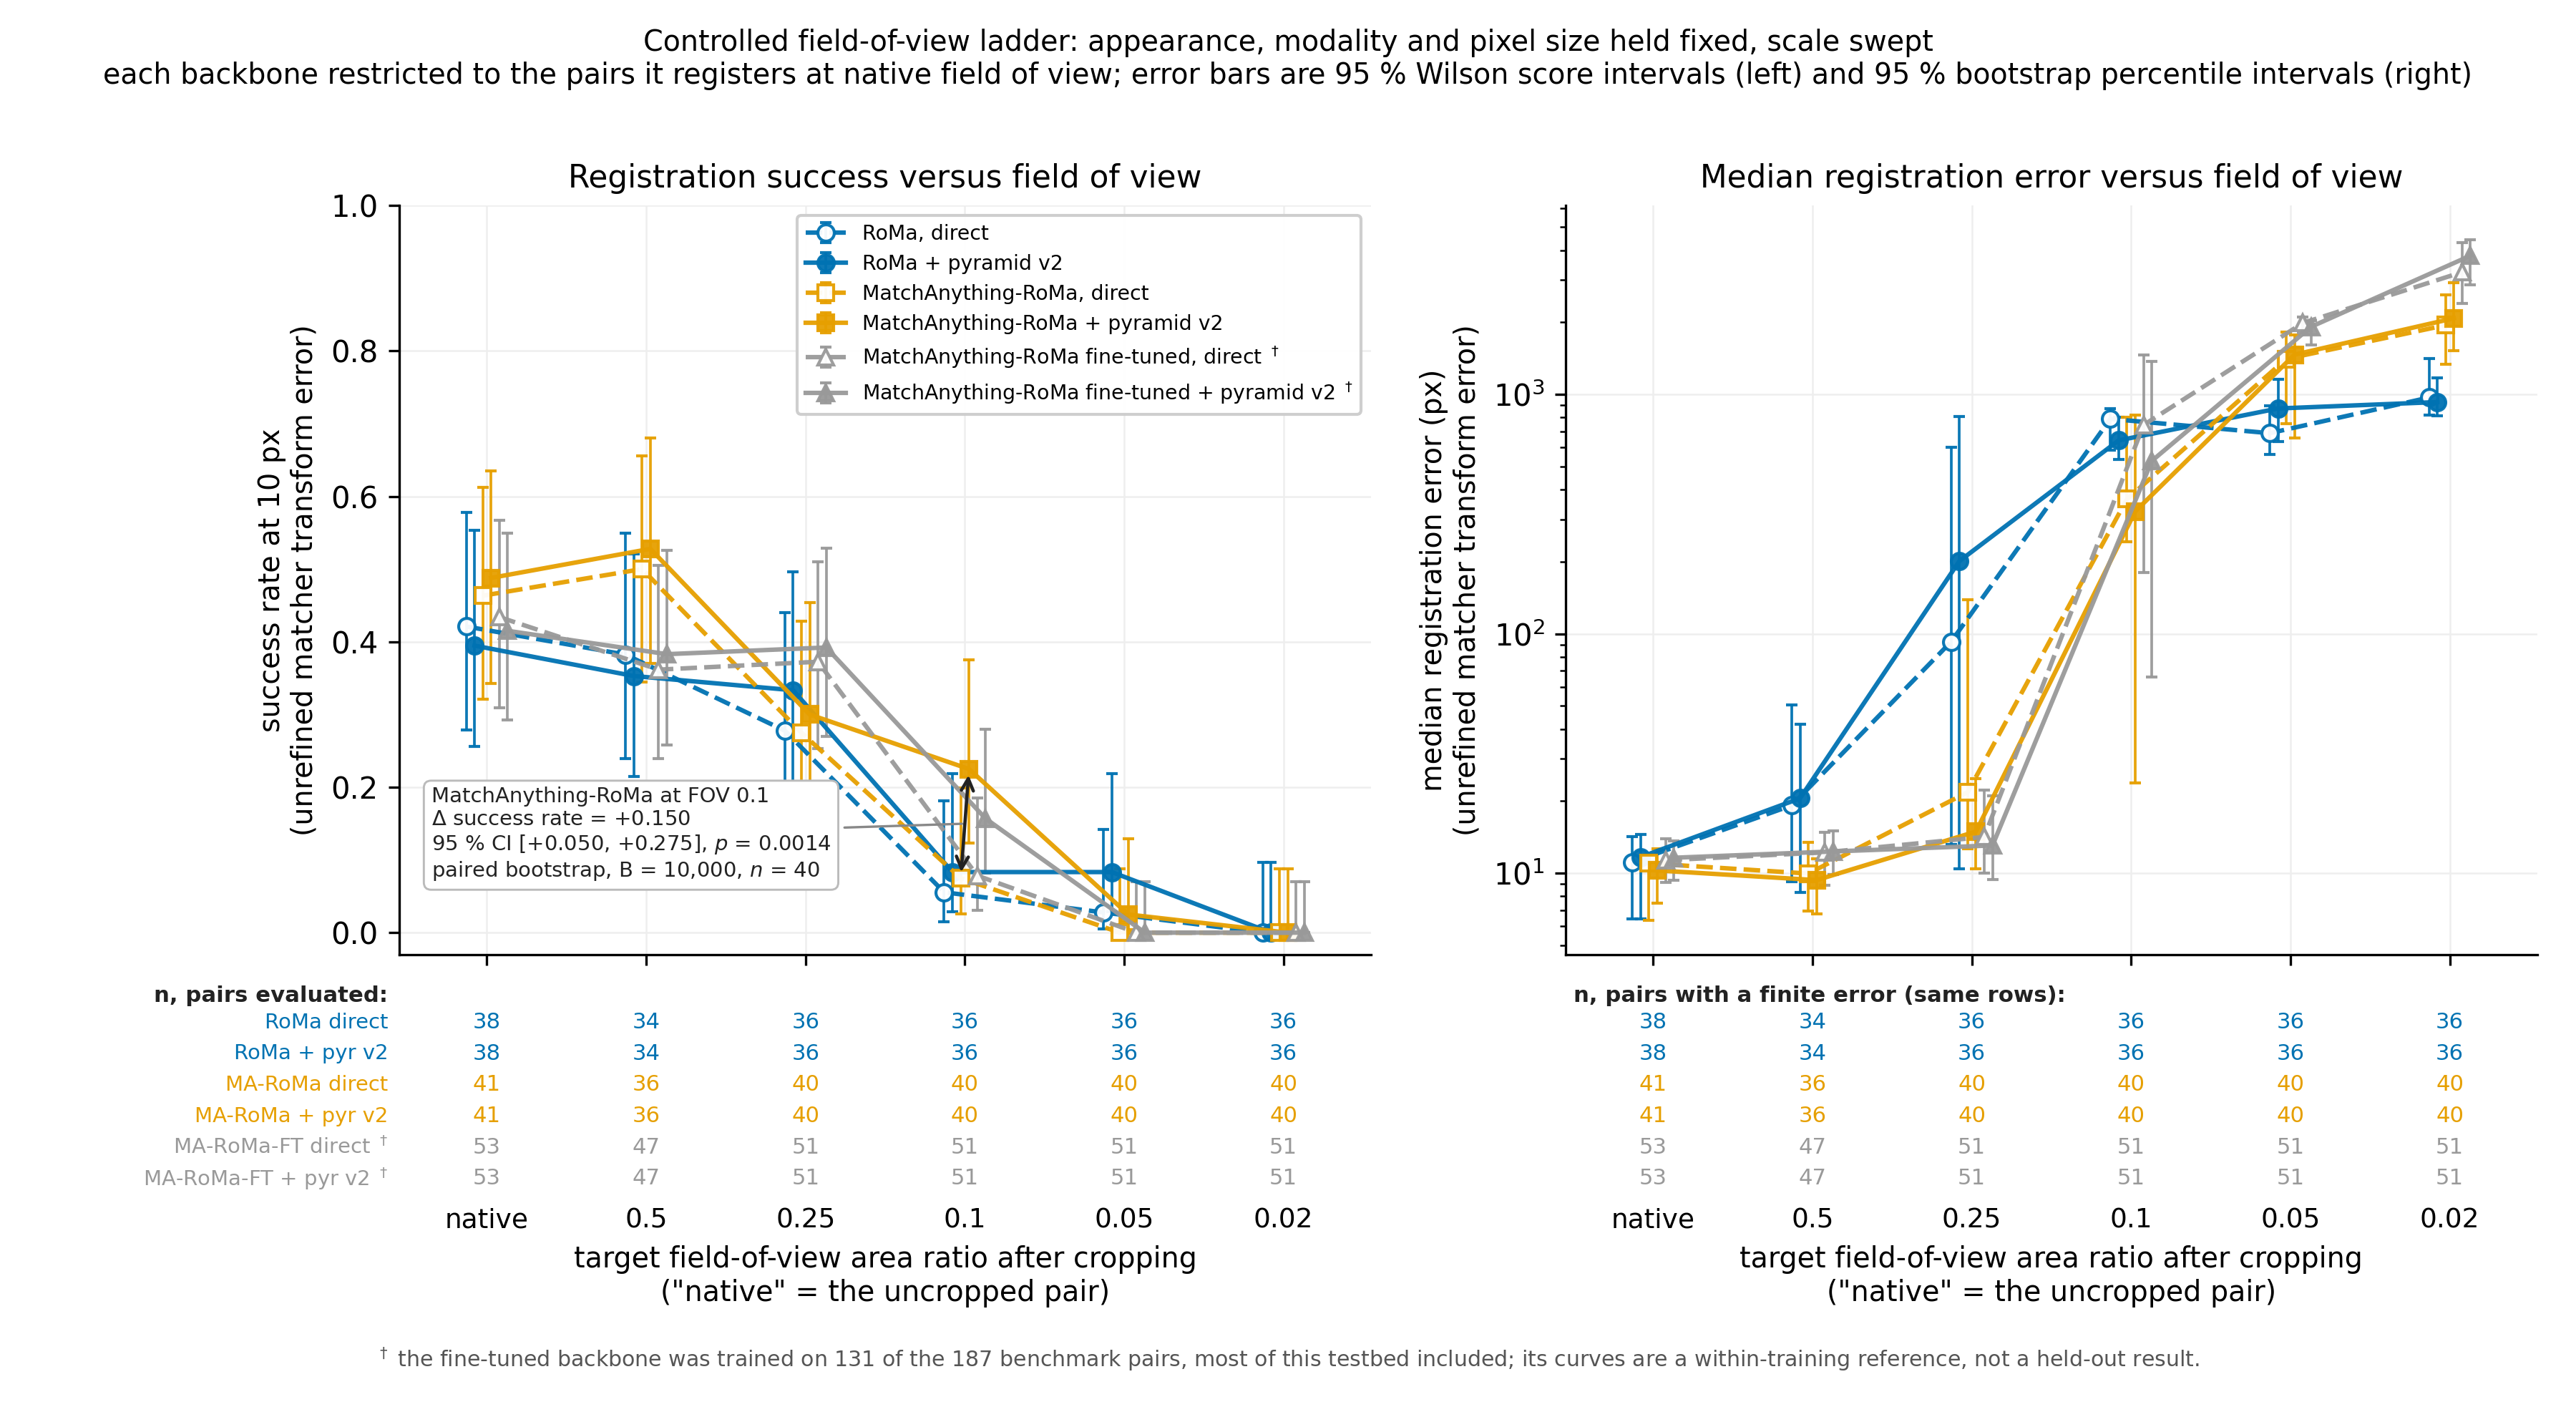
\includegraphics[width=\linewidth]{fov_ladder.png}
\caption{\textbf{Controlled FOV ladder, appearance held fixed, unrefined error.} Cropping base-matchable pairs to shrinking FOV ratios shows direct matching collapsing between the 0.25 and 0.1 rungs, while the verified wrapper restores success at 0.1 ($0.075\rightarrow0.225$, $p=0.0028$). The ladder is measured on the unrefined metric, which is the only one meaningful at every rung: at 10\,\% FOV, refinement has almost no inliers to work with and near-zero effect.}
\label{fig:fovladder}
\end{figure}

\section{Isolating appearance}
\label{sec:appearance}

\subsection{The backbone is the largest off-the-shelf lever, and it is not significant}

MatchAnything's released RoMa checkpoint is key-for-key compatible with the \texttt{roma\_outdoor} architecture (603/603 tensors, all retrained), so it drops into the identical pipeline with no code changes. Swapping it for stock RoMa is the largest single off-the-shelf change we found, and on the unrefined metric it is not statistically significant: SR@10 $0.091\rightarrow0.107$, $\Delta=+0.016$, 95\,\% CI $[-0.011,+0.043]$, $p=0.33$. Median error is unchanged ($+0.8$\,px, $p=0.86$). Under the refined metric the same contrast reads $+0.032$, $p=0.035$ (Section~\ref{sec:metric}).

The stratum breakdown (Table~\ref{tab:strata}) shows where the nominal gain sits: entirely in the ${\ge}0.5$ stratum, $15/126\rightarrow19/126$. Cross-modal training repairs appearance on pairs that were nearly matchable already; it does not reach pairs whose FOV is the binding constraint, where it registers $0/33$ against stock RoMa's $1/33$. This ordering --- MatchAnything-RoMa strongest overall --- agrees with the independent evaluation of \citet{durmaz2026foundation}. Our contribution is to locate the gain (high FOV), to bound it (not significant on unrefined error), and to show what it cannot reach.

\subsection{A directly measured appearance axis}

Both of the preceding sections lean on the claim that low FOV and appearance divergence are confounded on this benchmark. Rather than infer that by elimination, we measure it. For each pair we compute the normalised mutual information (NMI) between the two images on their GT-affine-aligned overlap region, which gives an appearance-similarity value per pair that is independent of any matcher, of any transform we fit, and of the error metric.

The confound is real: across all 187 pairs the correlation between $\log_{10}$ area ratio and NMI is $r=+0.215$ ($p=0.003$). Pairs with less field of view in common also share less mutual information, so on native pairs the two axes cannot be separated. But the relationship is not monotone, and we report this because it limits how the correlation may be used: per-stratum median NMI runs 0.0196, 0.0021, 0.1648, 0.0725 across the four bins, so the 0.25--0.5 stratum is in fact the \emph{most} mutually informative of the four, and the coefficient above is carrying a weak overall trend rather than a clean ordering.

\paragraph{The benchmark cannot rank scale against appearance.} Below area ratio 0.5 --- 61 pairs --- no zero-shot or wrapped configuration in this study registers more than three (Table~\ref{tab:strata}). A regime in which the best available method succeeds on 3 of 61 cases carries essentially no discriminative power: there is no room for one axis to explain variance that the other does not. We therefore state, as a finding about the benchmark rather than about the methods, that \textbf{AmalgaMatch has too little leverage below area ratio 0.5 to establish whether appearance or scale is the dominant constraint}, and that an earlier version of this work which claimed appearance dominance by elimination was not entitled to that conclusion.

\begin{figure}[t]
\centering
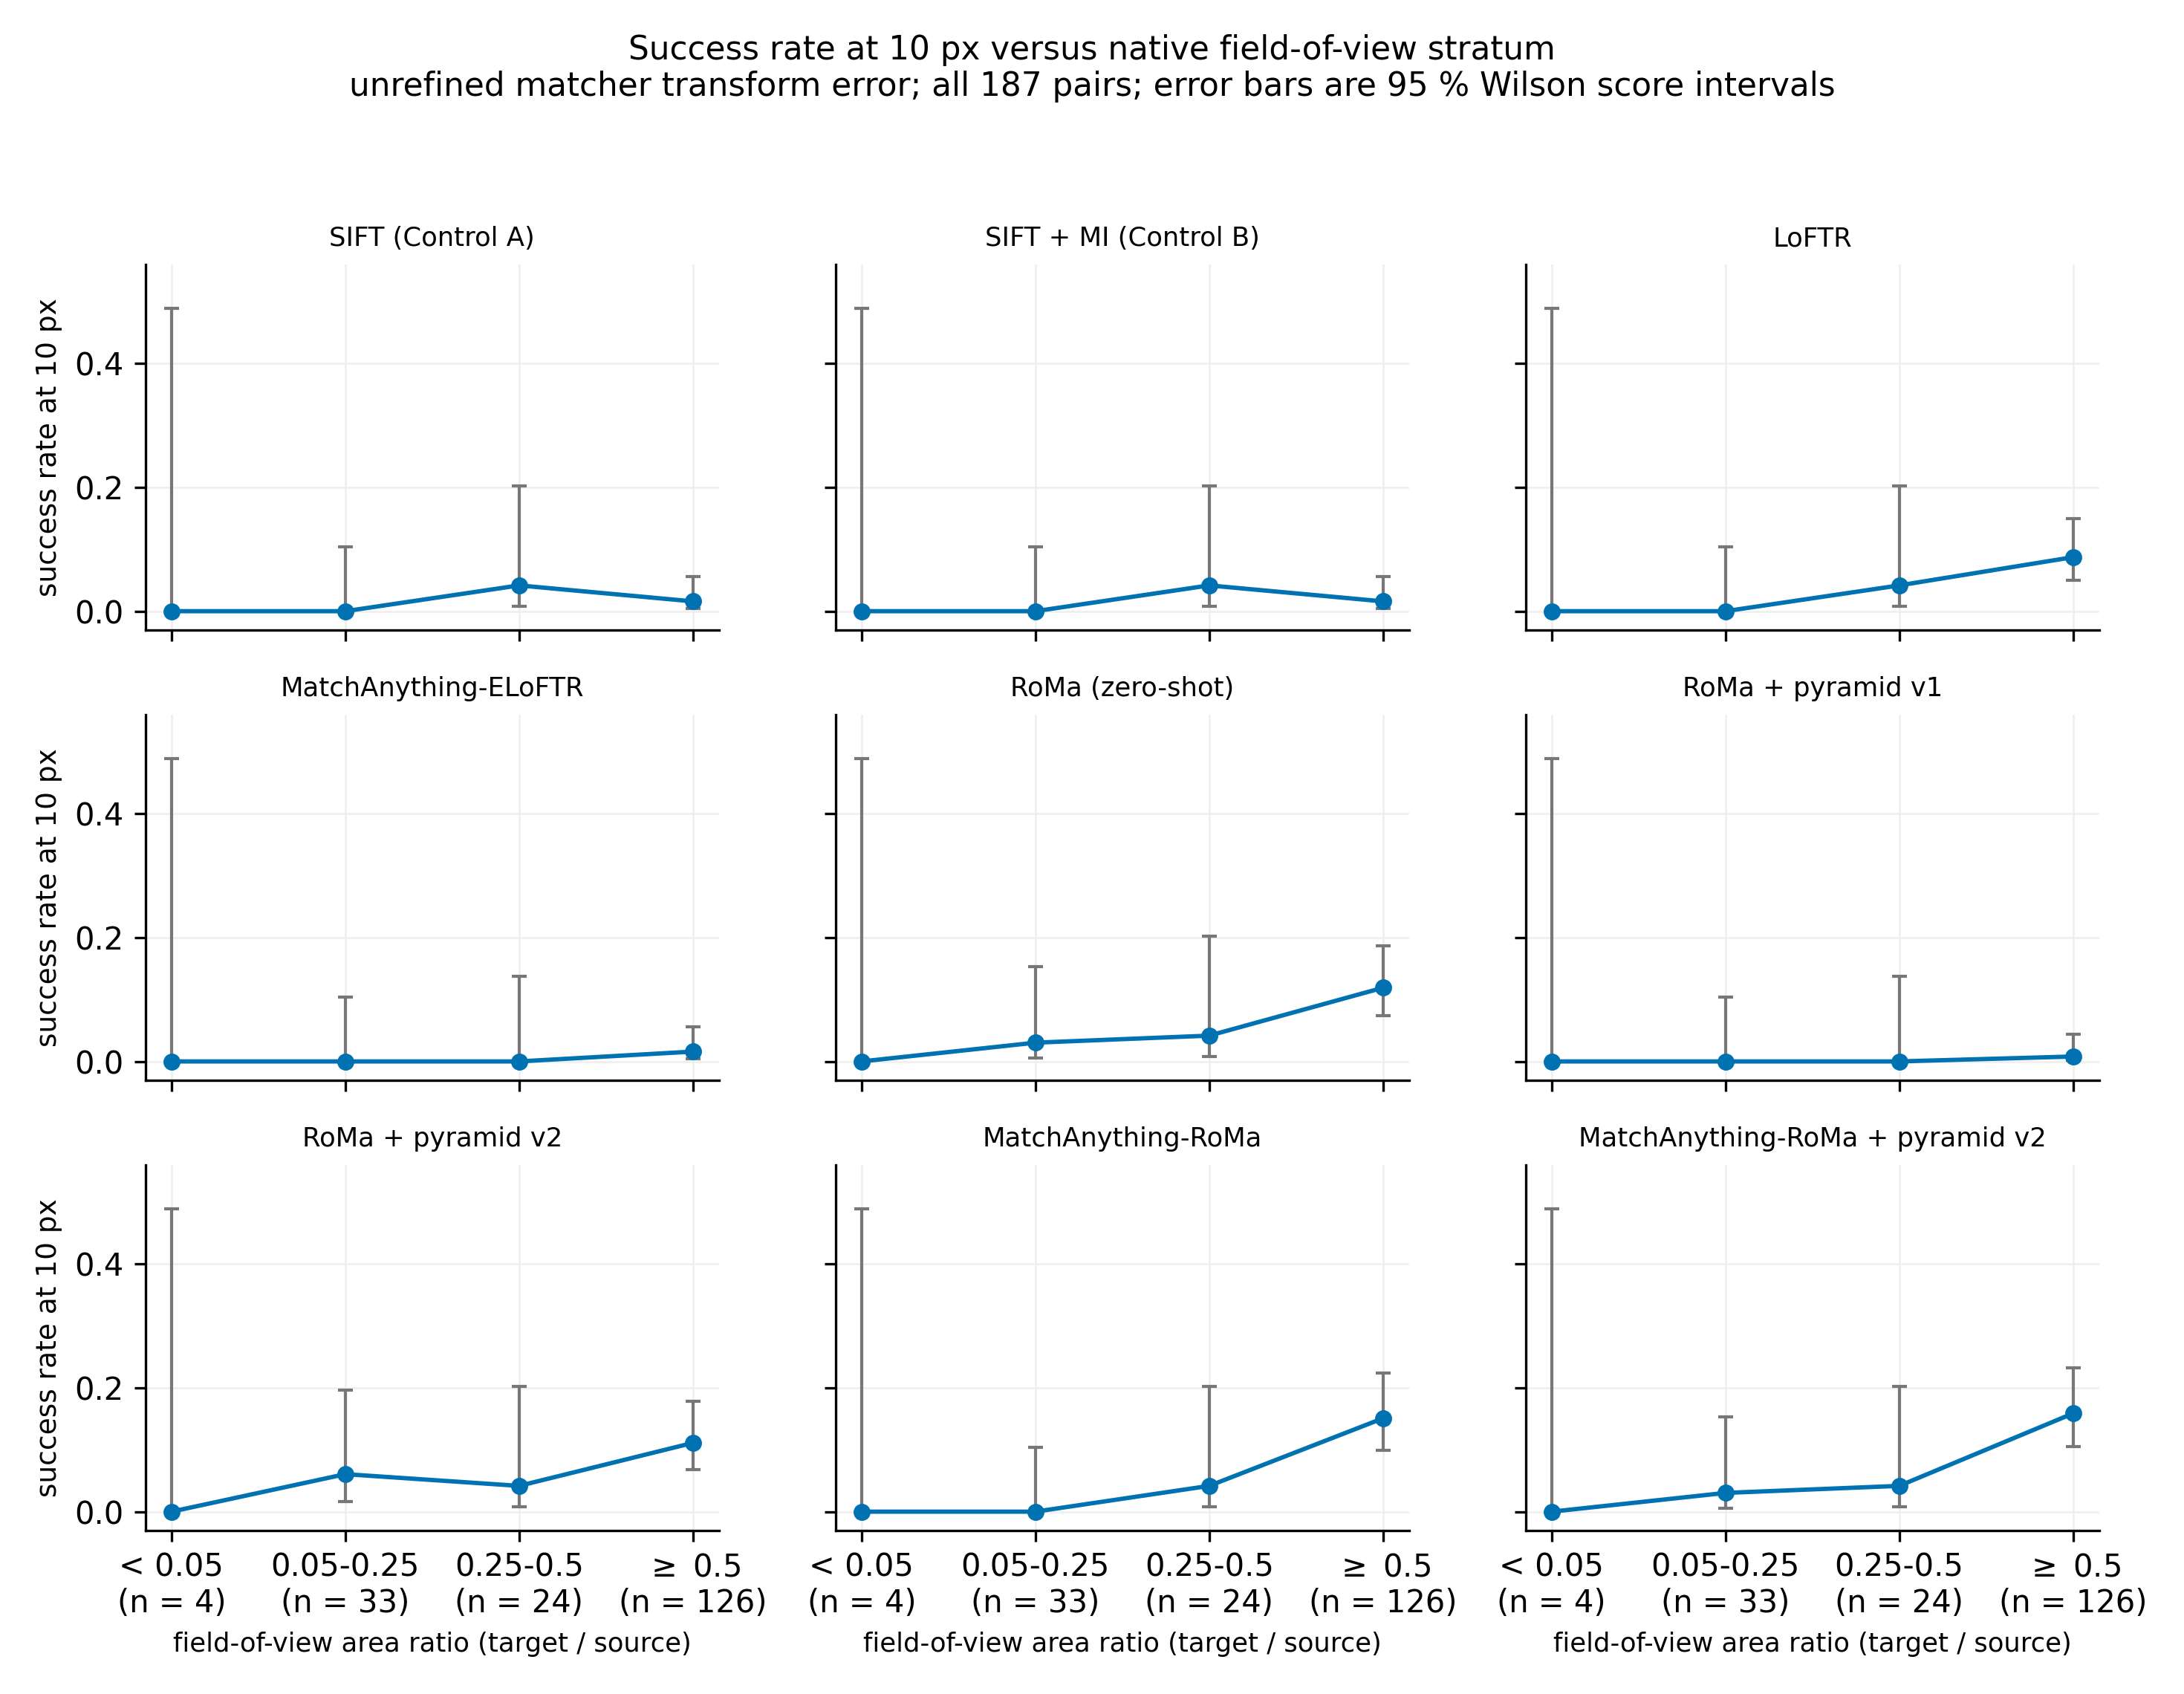
\includegraphics[width=\linewidth]{fov_curves_raw.png}
\caption{\textbf{Success at 10\,px versus native FOV stratum, unrefined error, with per-stratum $n$ and Wilson 95\,\% intervals.} The extreme-FOV stratum holds four pairs, so its interval is very wide and nothing may be read from its point estimate. Every configuration is at the floor there.}
\label{fig:fovcurves}
\end{figure}

\subsection{Domain fine-tuning trades in-distribution error for an untrained modality combination}
\label{sec:finetune}

The backbone swap suggests appearance is an operative constraint; fine-tuning attacks it directly. We fine-tune MatchAnything-RoMa's decoder on the materials domain, freezing the VGG+DINOv2 encoder in evaluation mode and training the ${\sim}100$M decoder parameters on a 131-pair training split (Appendix~\ref{app:impl}). In distribution the recipe works: median TEM error falls roughly $5\times$, consistently in direction across runs.

Out of distribution it costs. On the held-out 28-pair test split, averaged over eight training runs, SR@20 regresses from the zero-shot 0.393 to $0.264\pm0.019$ (Table~\ref{tab:finetune}). The regression is not diffuse. It falls on C103, the single subclass whose modality combination (SEM-SE against LOM height) our split leaves untrained, and within it on the four test pairs from two scenes. This is catastrophic forgetting \citep{kirkpatrick2017ewc} in the narrow sense of the term: the model loses a capability it had, on a combination it was never shown, while improving on what it was shown. We use the term at first mention with that scope stated, because it is often used more loosely.

We tested the cheapest available remedy. L2-SP \citep{li2018l2sp} adds $\tfrac{\lambda}{2}\lVert\theta_{\mathrm{dec}}-\theta_{\mathrm{dec}}^{0}\rVert^{2}$, anchoring the decoder to its zero-shot initialisation. Over eight runs it does not fix the regression: plain and anchored are statistically indistinguishable on every metric (Table~\ref{tab:finetune}), and on the one C103 scene that is recoverable at all the anchor is if anything less stable, retaining it in one of three runs against three of three for $\lambda=0$. The second C103 test scene is unrecoverable in every run and at every $\lambda$. That rules out an optimisation or anchor-strength explanation and is consistent with a modality-coverage gap, but the validation scene of the same untrained combination survives intact, so four pairs from two scenes cannot establish coverage as the cause.

\paragraph{Two protocol defects we disclose.} First, $\lambda$ was selected by held-out test-split retention rather than on validation, because the validation split cannot resolve the C103 damage. This biases every $\lambda$-conditioned effect size toward L2-SP and leaves the eight-run null unaffected --- the null is the result we report, and it is the one a biased selection procedure was least able to produce. A replication should select $\lambda$ on a fold constructed to contain the untrained modality combination. Second, these are independent runs, not seed replicates: only the augmentation sampler is seeded, so run-to-run variation includes nondeterministic GPU reduction order and is not reproducible from a seed alone. We report ``runs'' rather than ``seeds'' throughout for that reason.

\paragraph{An earlier draw, and why we report it.} An initial draw of three runs, whose checkpoints were deleted when the GPU instance was released, sat lower at direct SR@10 $0.095\pm0.021$. We tabulate it in full in Appendix~\ref{app:runs} rather than dropping it. It was not discarded for being unfavourable --- on SR@20 (0.297 against 0.264) and on median ED (46.0 against 47.9\,px) it is the \emph{better} draw, and only on SR@10 is it worse. The gap of about four pairs in 28 is roughly two standard errors of a 28-pair success rate, which is the scale of variation this test split can resolve.

\paragraph{A metric caveat specific to this section.} Table~\ref{tab:finetune} is scored on the TPS-refined error, not the unrefined error used everywhere else, because the per-pair outputs of the eight runs were not retained and only their summary rows survive; rescoring is therefore impossible. For the one fine-tuned run whose per-pair rows do survive, the held-out SR@20 regression is \emph{identical} under both metrics ($0.393\rightarrow0.250$ raw, $0.393\rightarrow0.250$ refined), so we do not expect this result to be metric-contingent in the way the wrapper and backbone contrasts are. We flag it rather than assume it.

\begin{table}[t]
\centering
\small
\begin{tabular}{llrrr}
\toprule
Method (8-run mean$\pm$SD) & Protocol & SR@10 & SR@20 & med ED (px) \\
\midrule
MatchAnything-RoMa (zero-shot)          & direct     & 0.214 & 0.393 & 83.5 \\
                                        & pyramid v2 & 0.214 & 0.393 & 69.1 \\
\midrule
MA-RoMa plain fine-tune ($\lambda{=}0$) & direct     & $0.236\pm0.019$ & $0.264\pm0.019$ & $49.6\pm3.7$ \\
                                        & pyramid v2 & $0.228\pm0.027$ & $0.264\pm0.019$ & $49.5\pm3.1$ \\
\midrule
MA-RoMa L2-SP ($\lambda{=}0.01$)        & direct     & $0.250\pm0.000$ & $0.268\pm0.019$ & $50.8\pm8.1$ \\
                                        & pyramid v2 & $0.245\pm0.023$ & $0.272\pm0.019$ & $50.2\pm6.6$ \\
\bottomrule
\end{tabular}
\caption{\textbf{Decoder-only fine-tuning on the held-out 28-pair test split: mean\,$\pm$\,SD over eight training runs.} Scored on TPS-refined ED --- the exception to this paper's primary metric, forced by non-retention of per-run outputs and discussed in the text. Zero-shot rows are deterministic. SR@5 is omitted as ${\approx}0$ at the ${\sim}10.3$\,px GT floor. Both protocols share per-run checkpoints. Plain and L2-SP are statistically indistinguishable on every metric, so the anchor is a zero-cost floor rather than a reliable improvement; both regress SR@20 against zero-shot while cutting in-distribution TEM median ED ${\sim}5\times$. The verified wrapper does not stack on the fine-tune (within-checkpoint SR@20 within $\pm0.01$). Per-run values are in Appendix~\ref{app:runs}.}
\label{tab:finetune}
\end{table}

\section{Refinement is not a neutral post-process}
\label{sec:metric}

Everything above is scored on the unrefined parametric error. Our original protocol scored it after TPS refinement, and we changed primary metric during revision. This section reports what that change does, because the effect is large enough to be a finding in its own right rather than a housekeeping note.

\paragraph{Both of our aggregate null results become significant under refinement.} The wrapper contrast on RoMa reads $\Delta=0.000$, $p=1.00$ unrefined and $+0.021$, 95\,\% CI $[+0.005,+0.043]$, $p=0.034$ refined. The backbone contrast reads $+0.016$, $p=0.33$ unrefined and $+0.032$, 95\,\% CI $[+0.005,+0.064]$, $p=0.035$ refined (Table~\ref{tab:contrasts}). Two publishable-looking results and two null results, from the same runs, the same pairs and the same bootstrap, differing only in whether an optional spline was applied before measuring.

\begin{table}[t]
\centering
\small
\begin{tabular}{llrrrl r}
\toprule
Contrast & metric & A & B & $\Delta$ & 95\,\% CI & $p$ \\
\midrule
RoMa + pyr.\ v2 vs.\ RoMa, SR@10   & unrefined & 0.0909 & 0.0909 & $+0.0000$ & $[-0.0160,+0.0160]$ & 1.000 \\
                                   & refined   & 0.0963 & 0.1176 & $+0.0214$ & $[+0.0053,+0.0428]$ & \textbf{0.034} \\
MA-RoMa vs.\ RoMa, SR@10           & unrefined & 0.0909 & 0.1070 & $+0.0160$ & $[-0.0107,+0.0428]$ & 0.334 \\
                                   & refined   & 0.0963 & 0.1283 & $+0.0321$ & $[+0.0053,+0.0642]$ & \textbf{0.035} \\
FOV ladder, MA-RoMa @ rung 0.1     & unrefined & 0.075\phantom{0}  & 0.225\phantom{0}  & $+0.150$\phantom{0}  & $[+0.050,+0.275]$\phantom{0} & \textbf{0.0028} \\
                                   & refined   & 0.025\phantom{0}  & 0.100\phantom{0}  & $+0.075$\phantom{0}  & $[+0.000,+0.175]$\phantom{0} & 0.087 \\
\bottomrule
\end{tabular}
\caption{\textbf{The same three contrasts under both error metrics.} Paired bootstrap, $B=10{,}000$, two-sided. The two native-pair contrasts are null unrefined and significant refined; the controlled ladder result is the reverse. No contrast is significant under both.}
\label{tab:contrasts}
\end{table}

\paragraph{Why we headline the unrefined metric.} The decisive reason is comparability, not effect size. A TPS refinement is only defined when the fit has enough surviving inliers to constrain a spline, so the refined column is populated for some configurations and not others. Coverage across Table~\ref{tab:headline}'s nine configurations ranges from 187/187 for every dense RoMa-family row down to 93/187 for LoFTR, 70/187 for Control A and \textbf{0/187 for Control B}. Where the column is blank the pipeline falls back to the unrefined value. A ``TPS-refined'' table therefore scores the dense rows entirely on refined error and the weak rows almost entirely on raw error: it is not one metric but two, interleaved by configuration, and part of the apparent gap between the strong and weak families is a difference in scoring rather than in registration. The unrefined metric scores all nine identically. Two further considerations point the same way. Refinement is an optional stage downstream of the object we are studying, which is the matcher and the wrapper; and it is not monotone --- across the 16 configurations in our result files, 13 configuration-pair combinations register below 10\,px unrefined and above it after refinement, so refinement destroys successes as well as creating them.

\paragraph{Consequences we accept.} Three claims in earlier versions of this work do not survive the change and we withdraw them. (i) The verified wrapper is not an accuracy improvement on native pairs; it is a collapse fix with a null aggregate effect. (ii) The backbone gain is suggestive, not established. (iii) A ``first non-zero result in the severe stratum'' claim was an artefact: under refinement the 0.05--0.25 stratum reads $0/33\rightarrow1/33$, which looks like a qualitative first; unrefined it reads $1/33\rightarrow2/33$, because the pair that supplies the ``zero'' is one that direct RoMa already registers to 3.3\,px and that refinement then pushes to 37.5\,px. The wrapper gains one pair in that stratum either way. Only the from-zero framing was metric-manufactured.

\paragraph{The general hazard.} We think this generalises beyond our pipeline. Any evaluation with an optional post-processing stage whose applicability depends on the quality of the thing being evaluated will produce a metric that is silently non-uniform across configurations, and will tend to flatter methods whose outputs are dense enough for the stage to fire. Refinement stages, outlier filters, and fallback heuristics all have this character. Our recommendation is narrow and cheap: report post-processing coverage per configuration alongside the metric, and check headline contrasts with the stage disabled. Had we done so at first submission, three of our claims would have been stated differently.

\begin{figure}[t]
\centering
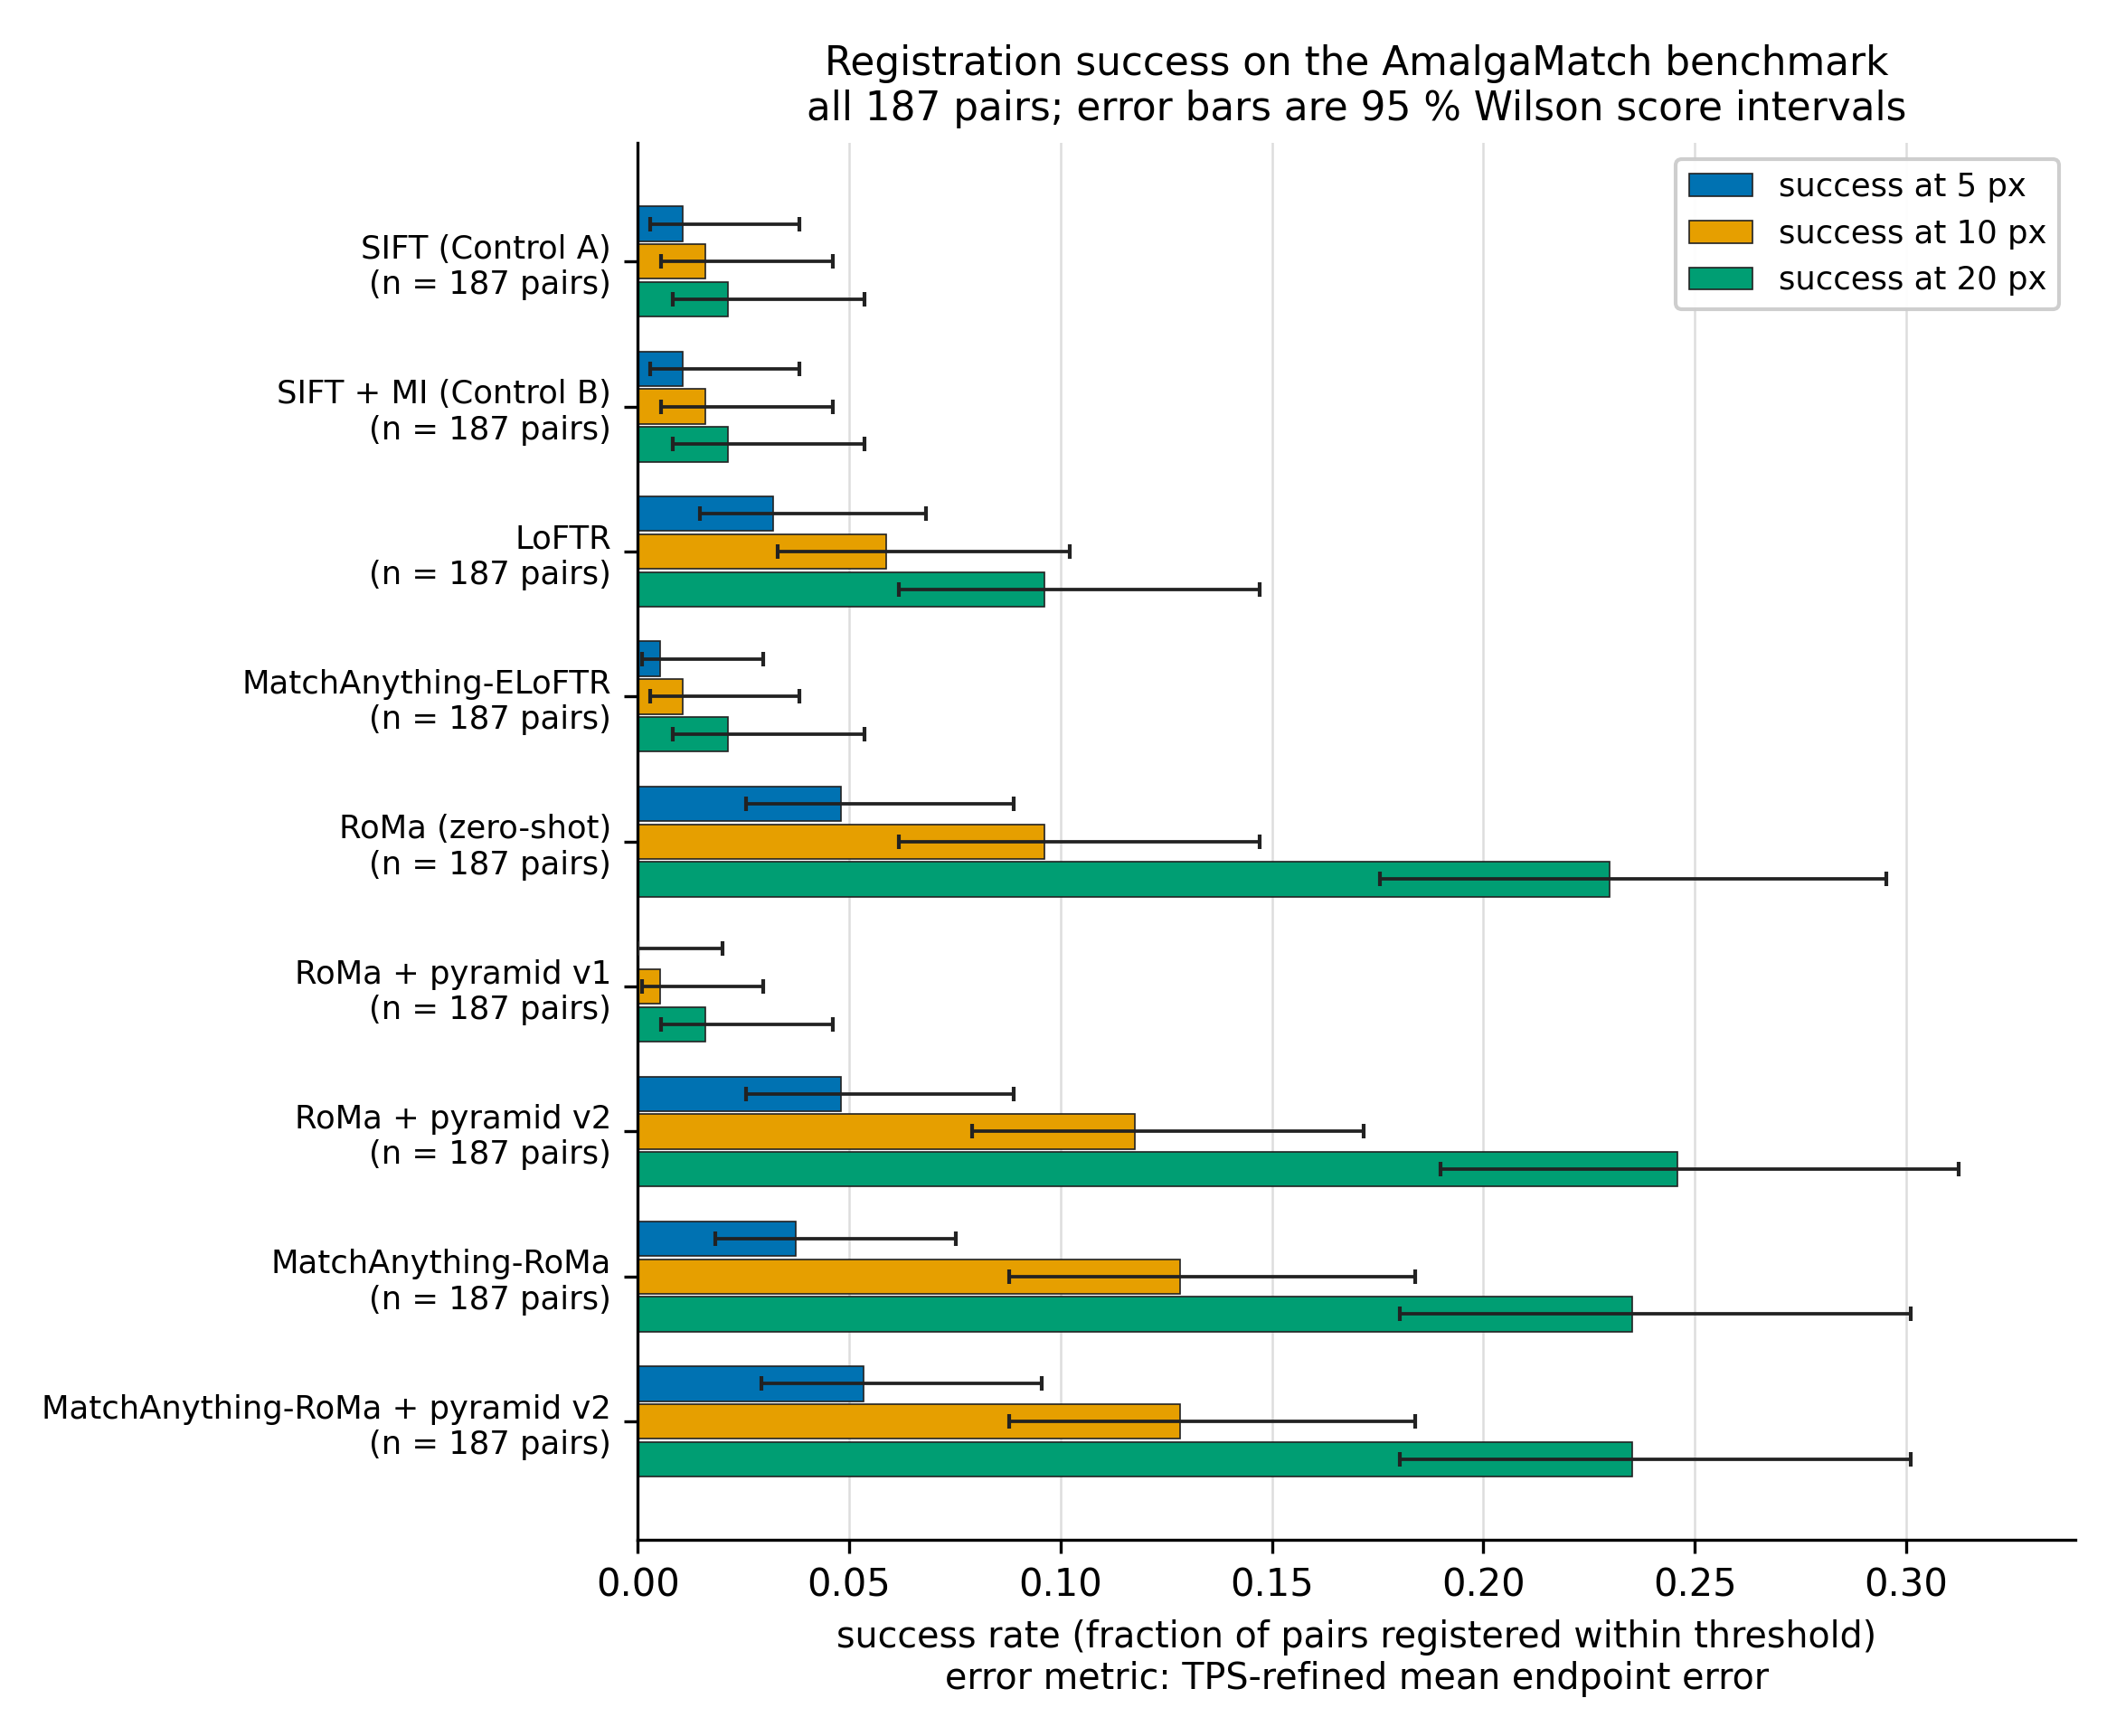
\includegraphics[width=0.92\linewidth]{sr_bars.png}
\caption{\textbf{The same nine configurations under the TPS-refined metric.} Compare Figure~\ref{fig:srbars}. The dense rows separate more here than they do unrefined, and part of that separation is the coverage artefact described in Section~\ref{sec:metric}: the four RoMa-family rows have 187/187 coverage while Control B has 0/187 and is scored entirely on the fallback.}
\label{fig:metric}
\end{figure}

\section{Hypothesis verdicts}
\label{sec:verdicts}

\textbf{H1 (${\ge}35\,\%$ relative gain at FOV\,${\le}\,5\,\%$): refuted, decisively and on both metrics.} Every configuration registers 0 of 4 pairs in the extreme-FOV stratum. No wrapper we built moves that number, and with $n=4$ the stratum could not have supported the claim even had it.

\textbf{H2 (RoMa's dense flow tolerates partial overlap better than the ELoFTR family at low FOV): supported, weakly.} RoMa beats MatchAnything-ELoFTR in aggregate (SR@10 0.091 against 0.011) and in each stratum where either registers anything: 1/33 against 0/33 at 0.05--0.25, 1/24 against 0/24 at 0.25--0.5. The direction is consistent, but the low-FOV evidence is a single pair, and we would not defend the claim on that alone.

\textbf{H3 (affine suffices; homography adds nothing): supported as stated, with one caveat we did not anticipate.} Among the 118 well-registered pairs across all zero-shot backbones (unrefined error below 20\,px), the BIC-style selector chooses affine on 82 (69\,\%) and homography on 36 (31\,\%). Affine is sufficient for roughly seven pairs in ten, which is the claim. The caveat is that the pairs on which the selector does reach for a homography are the \emph{more} accurate ones (median ED 6.5 against 11.3\,px for affine-selected), so we cannot add, as an earlier version of this work did, that homography confers no accuracy advantage. That comparison conditions on the selector's own decision and licenses no causal reading in either direction; separating the two would require fitting both families on every pair and comparing, which we did not do.

\section{Limitations}

\paragraph{The negative results are bounded by the benchmark, not by the mechanism.} Sections~\ref{sec:v2} and~\ref{sec:appearance} report nulls on native pairs, and Section~\ref{sec:ladder} shows the wrapper mechanism working when scale is isolated. The correct reading is that AmalgaMatch has 126 of 187 pairs at area ratio ${\ge}0.5$ and 4 below 0.05, so it is not an instrument for measuring FOV-adaptation methods. A benchmark stratified for FOV, with appearance controlled, would settle in one experiment what we could only approach by construction.

\paragraph{Ladder denominators are not equal.} Base-matchability is per backbone, so the three ladders rest on different and partly training-enriched pair sets (38, 41, 53). Cross-backbone comparisons read off the ladder are not like-for-like. The wrapper contrast, which is within-backbone, is unaffected, and its direction is preserved on held-out pairs for both backbones tested, though with different force: for zero-shot MatchAnything-RoMa it strengthens ($0.045\rightarrow0.227$, $p=0.023$), while for the fine-tuned backbone the direction holds but significance does not ($0.111\rightarrow0.278$, $p=0.077$, $n=18$).

\paragraph{Monotonicity is narrower than it sounds.} The verifier is monotone in its own mutual-information score, not in GT error. Per pair, the wrapper raises refined error on 94 of 187 pairs, materially on 22, with a worst case of $60.6\rightarrow1481.7$\,px. What it reliably avoids is losing threshold crossings, not regressing in error.

\paragraph{Not reproducible from the released files.} The per-run values of three fine-tuning runs, and the per-scene C103 readouts from the deleted checkpoints, cannot be regenerated. Everything else in this paper regenerates from the released result files.

\paragraph{Single benchmark, single domain.} Every measurement here is on AmalgaMatch. The non-abstention argument of Section~\ref{sec:v1} is analytic and should transfer to any non-abstaining matcher under any pyramid; we have not tested that, and it is the most valuable replication this work invites.

\section{Conclusion}

Wrapping a pretrained dense matcher in a pyramid is an appealing, training-free answer to extreme field-of-view mismatch, and the direct version of it does not work --- not because of tuning, but because dense matchers cannot abstain, so every non-overlapping tile contributes confident noise and robust estimation loses its consensus. A verified coarse-to-fine design repairs that, and on a controlled ladder where scale is the only variable it triples success at 10\,\% field of view. On the native benchmark it buys nothing, because that benchmark almost never presents scale as an isolated problem: its low-FOV pairs are also its most appearance-divergent, and it carries too little leverage in that regime to say which constraint dominates. We report both outcomes, and we report that the choice of whether to score before or after an optional refinement stage was, on our data, sufficient to turn two null results into significant ones --- which is why we headline the metric that scores every configuration the same way.

\subsubsection*{Reproducibility statement}

The evaluation harness, wrapper implementations, FOV-ladder construction, fine-tuning trainer with L2-SP, and every analysis script are released, together with the per-pair result files from which all tables and figures regenerate. Anonymised code is available at \url{https://anonymous.4open.science/r/correlative-microscopy-alignment} for review; a permanent archived release will be linked at camera-ready. The AmalgaMatch dataset is public \citep{durmaz2026amalgamatch}. Section~\ref{sec:setting} states the statistical protocol; the bootstrap is seeded and its seed is in the released scripts. The exceptions listed under Limitations --- per-run values for three fine-tuning runs and per-scene C103 readouts from non-retained checkpoints --- are the only quantities in this paper that cannot be regenerated from the release.

\bibliographystyle{tmlr}
\bibliography{references}

\appendix

\section{Implementation details}
\label{app:impl}

\paragraph{Backbones and weights.} We evaluate SIFT \citep{lowe2004sift}, LoFTR \citep{sun2021loftr}, the MatchAnything-ELoFTR configuration \citep{wang2024efficientloftr,he2025matchanything}, RoMa \citep{edstedt2024roma}, and MatchAnything-RoMa \citep{he2025matchanything}. RoMa couples frozen DINOv2 features \citep{oquab2024dinov2} with a fine-feature ConvNet and a match-classification decoder. The released MatchAnything-RoMa checkpoint is key-for-key compatible with the \texttt{roma\_outdoor} architecture (603/603 tensors), so it loads into the identical pipeline without modification.

\paragraph{Robust fitting.} Correspondences are fed to MAGSAC++ \citep{barath2020magsac}, a marginalising estimator in the RANSAC lineage \citep{fischler1981ransac} that replaces a hard inlier threshold with marginalisation over noise scale, at a 5.5\,px reprojection threshold. Both a 6-DoF affine and an 8-DoF homography are fit and selected by a BIC-style penalty on inlier residuals. The selected transform is optionally refined on its inliers with a thin-plate spline \citep{bookstein1989tps}; Section~\ref{sec:metric} covers the consequences. Matches are capped at $10^4$ per matcher invocation, a cap RoMa reaches on every pair; pyramid modes pool across invocations and are not capped in aggregate.

\paragraph{Pyramid wrappers.} Pyramid v1 tiles the source into a sliding-window pyramid at 50\,\% overlap whose levels match the target's nominal physical resolution, matches each tile, back-projects and pools all correspondences, then fits one global transform. Pyramid v2 computes a direct match and incumbent transform first, then evaluates candidate stages (tile search over the scaled source grid, then zoom refinement on the best-scoring region) only on weak direct support, accepting a candidate only if a mutual-information-on-overlap verifier improves on the incumbent. Ablations cover iterated versus single zoom and certainty gating at 0.5.

\paragraph{FOV-ladder construction.} For each backbone we take its base-matchable pairs (direct mean ED ${<}20$\,px) and crop the target to absolute area ratios $\{0.5,0.25,0.1,0.05,0.02\}$, holding appearance, modality and pixel size fixed. Full GT is retained so that out-of-crop correspondences test extrapolation of the fitted transform. The fine-tuned-backbone ladder is restricted to a fixed 63-pair testbed (39 train, 13 validation, 11 test) so that direct rows do not expand the eligible set.

\paragraph{Domain fine-tuning and L2-SP.} Fine-tuning is decoder-only: the VGG+DINOv2 encoder is held in evaluation mode with normalisation statistics fixed while ${\sim}100$M decoder parameters train. Supervision densifies sparse GT correspondences into an $A\rightarrow B$ warp via thin-plate splines and supervises inside the GT-support region under a sparse-GT-robust loss, with FOV-crop and photometric augmentation. Optimisation is AdamW at $2\times10^{-5}$ for 1500 steps; the checkpoint is selected by minimum validation median ED, which chose step 900 of 1500 (validation median 17.5 against 21.7\,px zero-shot). The anchored variant adds $\tfrac{\lambda}{2}\lVert\theta_{\mathrm{dec}}-\theta_{\mathrm{dec}}^{0}\rVert^{2}$ with $\lambda\in\{0,0.01,0.1,1.0\}$ swept. Only the augmentation sampler is seeded.

\paragraph{Appearance axis.} For each pair we warp the target into source coordinates under the GT-implied global affine, take the valid overlap region, quantise both images to 64 grey levels, and compute normalised mutual information over that region. The measure uses no matcher output and no fitted transform.

\section{Per-run fine-tuning results}
\label{app:runs}

Table~\ref{tab:seeds} gives per-run values for both draws on the 28-pair test split, scored on TPS-refined ED for the reason given in Section~\ref{sec:finetune}. Draw A is the earlier, non-retained draw of three runs whose checkpoints were deleted when the GPU instance was released; we tabulate it in full so that both draws can be compared directly rather than asking the reader to trust a summary. Draw B runs 1--3 also contribute to the Table~\ref{tab:finetune} aggregate, but their per-run values were not preserved and are recoverable only by arithmetic from the aggregate, so we do not tabulate them as measurements.

Across the five tabulated draw-B runs, SR@10 spans 0.214--0.250 for the plain fine-tune and is constant at 0.250 for L2-SP, while SR@20 spans 0.250--0.286 for both. Median ED differs in scatter rather than central tendency (plain 47.1--49.3, L2-SP 43.4--70.2\,px, the L2-SP range widened by a single high-residual run). No per-run separation supports calling L2-SP an improvement.

\begin{table}[ht]
\centering
\small
\begin{tabular}{llrrrr}
\toprule
Draw & Config & Run & SR@10 & SR@20 & med ED (px) \\
\midrule
A (not retained) & plain fine-tune ($\lambda{=}0$) & 1 & 0.107 & 0.321 & 48.9 \\
A (not retained) & plain fine-tune ($\lambda{=}0$) & 2 & 0.071 & 0.321 & 41.6 \\
A (not retained) & plain fine-tune ($\lambda{=}0$) & 3 & 0.107 & 0.250 & 47.6 \\
A (not retained) & L2-SP ($\lambda{=}0.01$)        & 1 & 0.107 & 0.286 & 52.5 \\
A (not retained) & L2-SP ($\lambda{=}0.01$)        & 2 & 0.107 & 0.286 & 52.9 \\
A (not retained) & L2-SP ($\lambda{=}0.01$)        & 3 & 0.071 & 0.250 & 63.5 \\
\midrule
B & plain fine-tune ($\lambda{=}0$) & 4 & 0.250 & 0.286 & 48.3 \\
B & plain fine-tune ($\lambda{=}0$) & 5 & 0.214 & 0.250 & 47.5 \\
B & plain fine-tune ($\lambda{=}0$) & 6 & 0.250 & 0.250 & 49.3 \\
B & plain fine-tune ($\lambda{=}0$) & 7 & 0.214 & 0.286 & 47.2 \\
B & plain fine-tune ($\lambda{=}0$) & 8 & 0.214 & 0.250 & 47.1 \\
B & L2-SP ($\lambda{=}0.01$)        & 4 & 0.250 & 0.250 & 70.2 \\
B & L2-SP ($\lambda{=}0.01$)        & 5 & 0.250 & 0.286 & 50.2 \\
B & L2-SP ($\lambda{=}0.01$)        & 6 & 0.250 & 0.250 & 43.4 \\
B & L2-SP ($\lambda{=}0.01$)        & 7 & 0.250 & 0.250 & 50.6 \\
B & L2-SP ($\lambda{=}0.01$)        & 8 & 0.250 & 0.286 & 47.8 \\
\bottomrule
\end{tabular}
\caption{\textbf{Per-run direct-match results for both draws} (28-pair test split, TPS-refined ED).}
\label{tab:seeds}
\end{table}

\section{Metric sensitivity: full tables}
\label{app:metric}

\paragraph{TPS coverage by configuration.} The fraction of the 187 pairs for which the refinement stage produced a value, the remainder falling back to the unrefined error. This is the comparability defect of Section~\ref{sec:metric}: 187/187 for RoMa (zero-shot), RoMa + pyramid v2, MatchAnything-RoMa and MatchAnything-RoMa + pyramid v2; 93/187 for LoFTR; 82/187 for MatchAnything-ELoFTR; 72/187 for RoMa + pyramid v1; 70/187 for Control A; and 0/187 for Control B.

\paragraph{Successes destroyed by refinement.} Across the 16 configurations in the released result files, 13 configuration-pair combinations register below 10\,px on the unrefined fit and at or above 10\,px after refinement. The largest single case is \texttt{eval\_5842WCu-Spalled\_SEM-SE\_SEM-BSE\_Multiscale\_0\#0} under RoMa direct, at 3.3\,px unrefined and 37.5\,px refined; that pair is the one discussed in Section~\ref{sec:metric} whose disappearance manufactures the from-zero appearance of the low-FOV stratum.

\paragraph{Full ladder table under both metrics.} All rungs, both metrics, both the base-matchable and the held-out-restricted denominators, are released as \texttt{reports/metric\_sensitivity.md} and \texttt{results/metric\_sensitivity.csv}, regenerated by \texttt{scripts/metric\_sensitivity.py}.

\end{document}
